\documentclass{tufte-handout}

\usepackage{style}

\begin{document}
\tma{04}

%%%Question one
\begin{question}
    
    \[
    \textbf{A} = 
    \begin{pmatrix}
        4 & 7 & -2\\
    \end{pmatrix}
    \textbf{B} =
    \begin{pmatrix}
        1 & -3\\
        0 & 1\\
        3 & -1
    \end{pmatrix}
    \textbf{C} = 
    \begin{pmatrix}
        2 & 5\\
        -1 & 0
    \end{pmatrix}
    \]

    \qpart
    \qsubpart
    
    \begin{align*}
    \textbf{AB}
    &=
        \begin{pmatrix}
            4\cdot{1}+7\cdot{0}+\rb{-2}\cdot{2} & 4\cdot{\rb{-3}}+7\cdot{1}+-2\cdot{\rb{-1}}\\
        \end{pmatrix}\\[15pt]
    &=
        \begin{pmatrix}
            -2\\
            3
        \end{pmatrix}
    \end{align*}
        
\vspace{3cm}

    \qsubpart
    \textbf{BA} = This cannot be done, numbr of columns in \textbf{B} is not equal to the number of rows in \textbf{A}.

\clearpage

\qsubpart
    
\begin{align*}
\textbf{BC}
&= 
    \begin{pmatrix}
        1 & -3\\
        0 & 1\\
        3 & -1
    \end{pmatrix}
    \cdot{
        \begin{pmatrix}
            2 & 5\\
            -1 & 0
        \end{pmatrix}
    }\\[15pt]
&=
    \begin{pmatrix}
        1\cdot{2}+(-3)\cdot{(-1)} & 1\cdot{5}+(-3)\cdot{0}\\
        0\cdot{2}+1\cdot{(-1)} & 0\cdot{5}+1\cdot{0}\\
        3\cdot{2}+(-1)\cdot{(-1)} & 3\cdot{5}+(-1)\cdot{0}
    \end{pmatrix}\\[15pt]
&=
    \begin{pmatrix}
        2+3 & 5+0\\
        0-1 & 0+0\\
        6+1 & 15-0
    \end{pmatrix}\\[15pt]
&=
    \begin{pmatrix}
        5 & 5\\
        -1 & 0\\
        7 & 15
    \end{pmatrix}
\end{align*}

\vspace{5cm}

    \qsubpart
    
    \marginnote{\[ A^{2} = 
    \begin{pmatrix}
        a^{2}+bc & ab+bd\\
        ca + dc & cb+d^{2}
    \end{pmatrix} \]}

    \begin{align*}
    \mathbf{C}^{2} 
    &=
        \begin{pmatrix}
            2^{2}+ 5\cdot{-1} & 2\cdot{5}+ 5\cdot{0}\\
            -1\cdot{2} +0\cdot{-1} & -1\cdot{5} + 0^{2} 
        \end{pmatrix} \\[15pt]
    &=
        \begin{pmatrix}
            -1 & 10\\
            -2 & -5
        \end{pmatrix}
\end{align*}

\vspace{3cm}

    \qsubpart

    \begin{align*}
    \textbf{4BC-3B}
    &=
        \begin{pmatrix}
            4 & -12\\
            0 & 4\\
            8 & -4
        \end{pmatrix}
        \cdot{
            \begin{pmatrix}
                2 & 5\\
                -1 & 0
            \end{pmatrix}
        }
        -
        \begin{pmatrix}
            3 & -9\\
            0 & 3\\
            6 & -3
        \end{pmatrix}\\[15pt]
    &=
        \begin{pmatrix}
            4\cdot{2}+(-12)\cdot{(-1)} & 4\cdot{5}+\rb{-12}\cdot{0}\\
            0\cdot{2}+4\cdot{\rb{-1}} & 0\cdot{5}+4\cdot{0}\\
            8\cdot{2}+\rb{-4}\cdot{\rb{-1}} & 8\cdot{5}+\rb{-4}\cdot{0}
        \end{pmatrix}
        -
        \begin{pmatrix}
            3 & -9\\
            0 & 3\\
            6 & -3
        \end{pmatrix}\\[15pt]
    &=
        \begin{pmatrix}
            20 & 20\\
            -4 & 0\\
            16 & 20
        \end{pmatrix}
        -
        \begin{pmatrix}
            3 & -9\\
            0 & 3\\
            6 & -3
        \end{pmatrix}\\[15pt]
    &=
        \begin{pmatrix}
            17 & 29\\
            -4 & -3\\
            10 & 23
        \end{pmatrix}
    \end{align*}

\clearpage

\qpart

\marginnote{  
To find the inverse of a matrix}
\marginnote{\[ |\textbf{A}| = \frac{1}{ad-bc} \]}
\marginnote{\[ \begin{pmatrix}
    a & b\\
    c & d
\end{pmatrix}^{-1} = |A|\cdot\begin{pmatrix}
    d & -b\\
    -c & a
\end{pmatrix} \]}

\begin{align*}
    2x - 6y &= -12\\[8pt]
    3x - 7y &= 10\\[8pt]
\stext{In matrix notation \( \mathbf{AX} = \mathbf{B} \)}\\[8pt]
    \begin{pmatrix}
        2&\rb{-6}\\
        3&\rb{-7}
    \end{pmatrix}
    \cdot{
        \begin{pmatrix}
            x\\
            y
        \end{pmatrix}
    }
    &=
    \begin{pmatrix}
        -12\\
        10
    \end{pmatrix}\\[15pt]
\stext{Hence \( \mathbf{X} = \mathbf{A}^{-1}\mathbf{B} \)}\\[8pt]
    \begin{pmatrix}
        x\\
        y
    \end{pmatrix}
    &=
    \frac{1}{\rb{-7}2-\rb{-6}3}
    \cdot{
        \begin{pmatrix}
            \rb{-7} & 6\\
            \rb{-3} & 2
        \end{pmatrix}
    }
    \cdot{
        \begin{pmatrix}
            \rb{-12}\\
            10
        \end{pmatrix}
    }\\[15pt]
    &=
    \frac{1}{\rb{-14}+18}
    \cdot{
        \begin{pmatrix}
            -7\cdot{\rb{-12}}+6\cdot{10}\\
            -3\cdot{\rb{-12}}+2\cdot{10}
        \end{pmatrix}
    }\\[15pt]
    &=
    \frac{1}{4}
    \cdot{
        \begin{pmatrix}
            144\\
            56
        \end{pmatrix}
    }\\[15pt]
    &=
    \begin{pmatrix}
        36\\
        14
    \end{pmatrix}
\stext{therefore}
    x &= 36\\
    y &= 14
\end{align*}

\end{question}

\clearpage

%%%%Question two

\begin{question}
    
    \qpart

    \qsubpart
    \begin{center}
        \begin{tikzpicture}
            % Define vertices
            \Vertex[label=X,x=3,color=red,opacity=0.2]{X}
            \Vertex[label=A, x=0, y=-3, color=yellow,opacity=0.2]{A}
            \Vertex[label=B,x=6, y=-3,color=green!70!blue,opacity=0.2]{B}
            \Vertex[label=Y,x=9,color=blue,opacity=0.2]{Y}
            \Vertex[label=C,x=12, y=-3,color=orange,opacity=0.2]{C}
            
            % Define edges with labels
            \Edge[label=0.9,fontscale=2,position=above, color=red](X)(A)
            \Edge[label=0.1,fontscale=2,position=below, color=blue](Y)(A)
            \Edge[label=0.15,fontscale=2,position=above, color=red](X)(B)
            \Edge[label=0.85,fontscale=2,position=below, color=blue](Y)(B)
            \Edge[label=0.55,fontscale=2,position=above, color=red](X)(C)
            \Edge[label=0.45,fontscale=2,position=below, color=blue](Y)(C)
            
            % Add arrowheads manually using TikZ
            \draw[->-=0.5, thick, red] (X) -- (A);
            \draw[->-=0.8, thick, blue] (Y) -- (A);
            \draw[->-=0.7, thick, red] (X) -- (B);
            \draw[->-=0.6, thick, blue] (Y) -- (B);
            \draw[->-=0.7, thick, red] (X) -- (C);
            \draw[->-=0.5, thick, blue] (Y) -- (C);
            
        \end{tikzpicture}
    \end{center}
    
    \qsubpart\[
    \begin{pmatrix}
        0.9 & 0.1\\
        0.15 & 0.85\\
        0.55 & 0.45
    \end{pmatrix}
    \cdot{
        \begin{pmatrix}
            X\\
            Y
        \end{pmatrix}
    }
    \]
    
    \qsubpart
    
    \begin{align*}
    \stext{Given the power distribution matrix}\\
    A =
    \begin{pmatrix}
        0.9 & 0.1 \\
        0.15 & 0.85 \\
        0.55 & 0.45
    \end{pmatrix}
    \stext{and the total power consumption per city}\\
    B =
    \begin{pmatrix}
        700\\
        900\\
        800
    \end{pmatrix}\\[15pt]
    \stext{We can represent the system as}\\
    \begin{pmatrix}
        0.9 & 0.1 \\
        0.15 & 0.85 \\
        0.55 & 0.45
    \end{pmatrix} 
    \begin{pmatrix}
        X\\
        Y
    \end{pmatrix}
    &=
    \begin{pmatrix}
        700\\
        900\\
        800
    \end{pmatrix}\\[15pt]
    \stext{We compute the total contribution from each power station as}\\
    \begin{pmatrix}
        0.9\cdot700 + 0.15\cdot900 + 0.55\cdot800 \\
        0.1\cdot700 + 0.85\cdot900 + 0.45\cdot800
    \end{pmatrix}\\[15pt]
    &=
    \begin{pmatrix}
        630 + 135 + 440 \\
        70 + 765 + 360
    \end{pmatrix}\\[15pt]
    &=
    \begin{pmatrix}
        1205 \\
        1195
    \end{pmatrix}
    \stext{Thus, the total power supplied by each station is}
    X = \SI{1205}{\giga\watt\hour}, \quad Y = \SI{1195}{\giga\watt\hour}
\end{align*}

\vspace{5cm}

\qpart

\qsubpart
\begin{align*}
    \begin{pmatrix}
        0.2 & 0.6\\
        0.8 & 0.4
    \end{pmatrix}
\end{align*}

\qsubpart
\begin{align*}
    &\begin{pmatrix}
        0.2 & 0.6\\
        0.8 & 0.4
    \end{pmatrix}
    \cdot
    \begin{pmatrix}
        0.9 & 0.15 & 0.55\\
        0.1 & 0.85 & 0.45
    \end{pmatrix}\\[15pt]
    &=
    \begin{pmatrix}
        0.2\cdot0.9 + 0.6\cdot0.1 & 0.2\cdot0.15 + 0.6\cdot0.85 & 0.2\cdot0.55 + 0.6\cdot0.45\\
        0.8\cdot0.9 + 0.4\cdot0.1 & 0.8\cdot0.15 + 0.4\cdot0.85 & 0.8\cdot0.55 + 0.4\cdot0.45
    \end{pmatrix}\\[15pt]
    &=
    \begin{pmatrix}
        0.18 + 0.06 & 0.03 + 0.51 & 0.11 + 0.27\\
        0.72 + 0.04 & 0.12 + 0.34 & 0.44 + 0.18
    \end{pmatrix}\\[15pt]
    &=
    \begin{pmatrix}
        0.24 & 0.54 & 0.38\\
        0.76 & 0.46 & 0.62
    \end{pmatrix}
\stext{Town A’s fossil fuel dependency: } 0.9 \times 0.8 + 0.4 \times 0.1 = 0.76 = 76\%  
\stext{Town B’s fossil fuel dependency: } 0.15 \times 0.8 + 0.85 \times 0.4 = 0.46 = 46\%  
\stext{Town C’s fossil fuel dependency: } 0.55 \times 0.8 + 0.45 \times 0.4 = 0.65 = 65\%  
\stext{Since Town A has the highest percentage of power derived from fossil fuels (76\%), it is the most affected.}
\end{align*}

\end{question}

\clearpage

%%%%Question three

\begin{question}

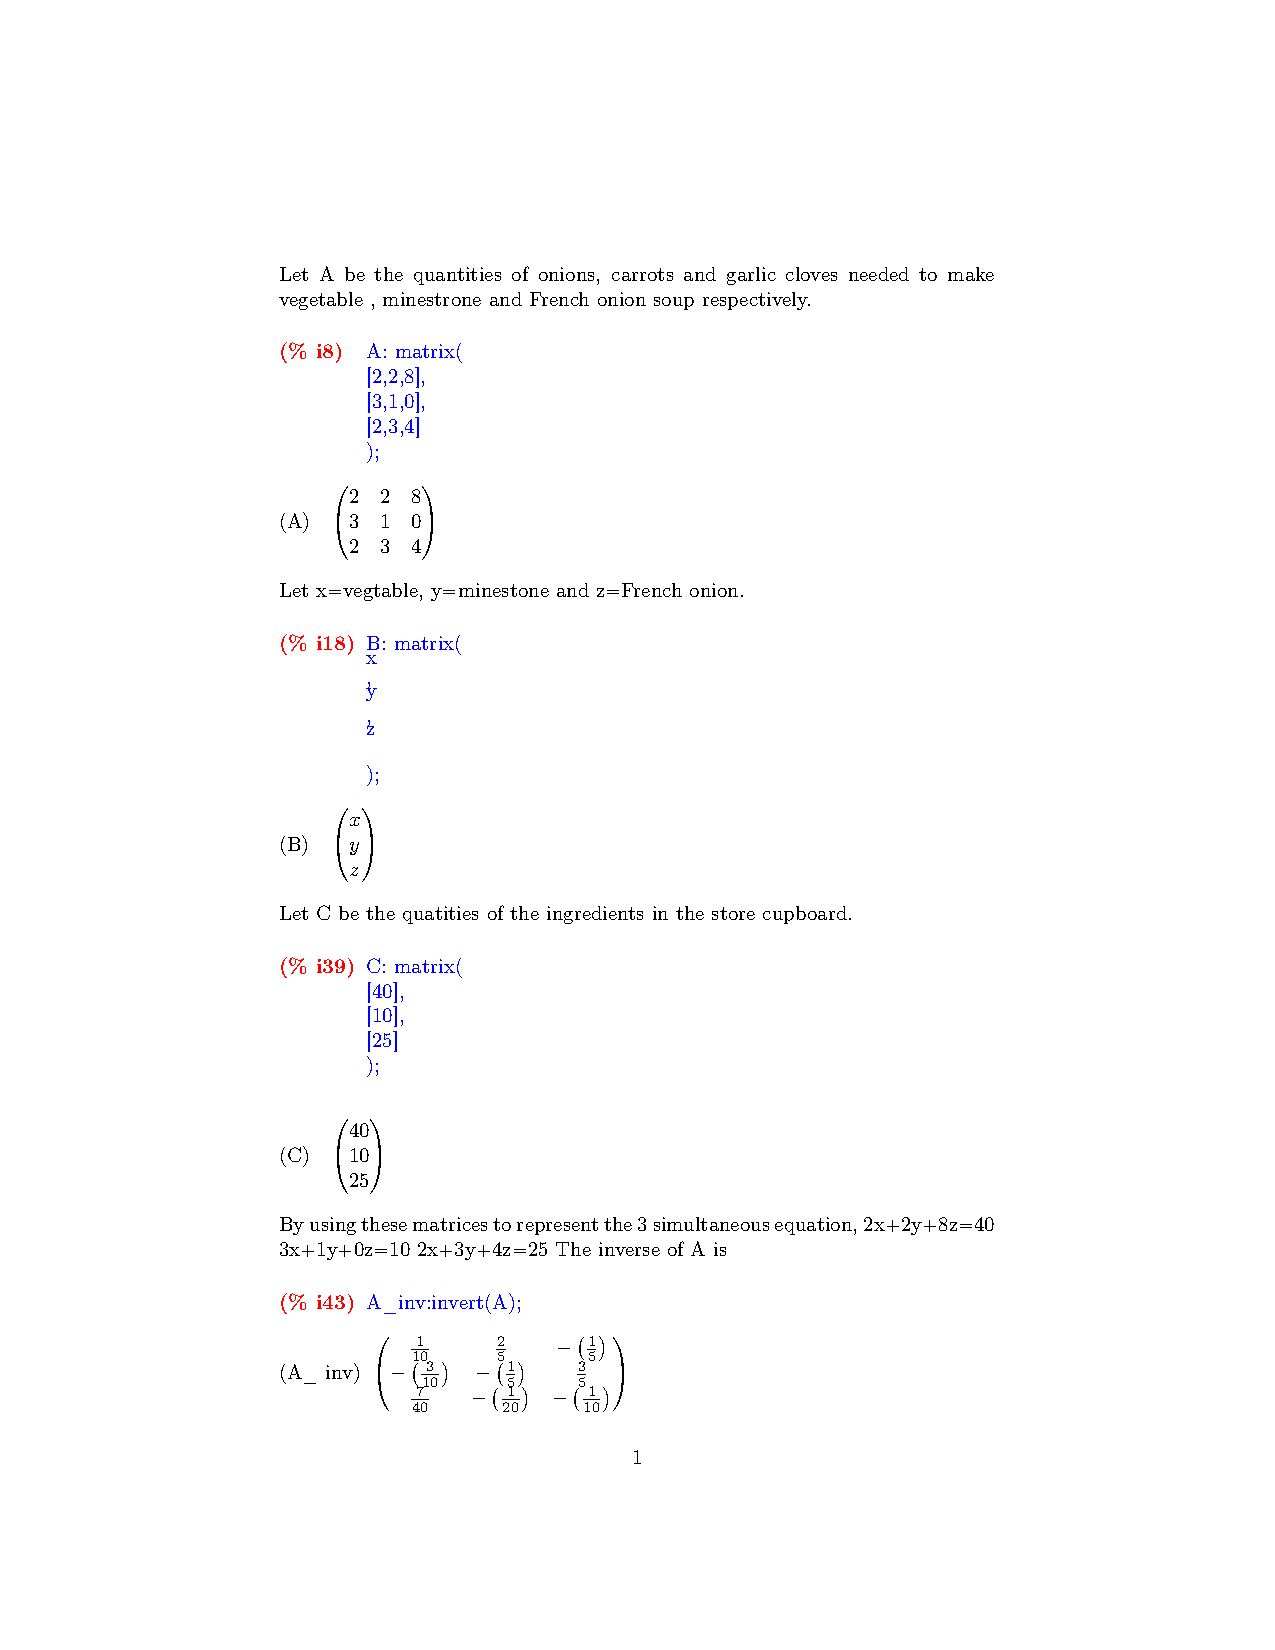
\includepdf[pages=-]{question_3wxmx.pdf}

\end{question}

\clearpage

%%%%Question four

\begin{question}

\begin{align*}
\stext{Let}\\
    x &= 0.273273273\ldots\\[8pt]
\stext{Then}\\
    1000x &= 273.273273273\ldots\\[8pt]
\stext{Subtracting the first equation from the second gives}\\
    999x &= 273\\   
\stext{Therefore}\\
    x &= \frac{273}{999}\\[8pt]
\stext{Simplifying the fraction gives}\\
    x &= \frac{91}{333}
\end{align*}

\end{question}

\clearpage

%%%Question five
\begin{question}

    Given:
    \[ \left(\frac{x}{4} - 5\right)^{7} \]
    
    We use the general formula for the binomial expansion:
    \begin{align*}
    ( a + b )^{n} &= \sum_{r=0}^{n} \binom{n}{r} a^{n-r} b^r, \\
    \binom{n}{r} = \frac{n!}{r!(n-r)!}.
    \end{align*}
    \vspace{3cm}   
    Substituting \( a = \frac{x}{4} \), \( b = -5 \), and \( n = 7 \):
    \begin{align*}
        (a + b)^n &= \sum_{r=0}^{7} \binom{7}{r} \left(\frac{x}{4}\right)^{7-r} (-5)^r \\
        &= \binom{7}{0}\left(\frac{x}{4}\right)^{7} + \binom{7}{1}\left(\frac{x}{4}\right)^{6}(-5) + \binom{7}{2}\left(\frac{x}{4}\right)^{5}(-5)^2 \\
        &\quad + \binom{7}{3}\left(\frac{x}{4}\right)^{4}(-5)^3 + \binom{7}{4}\left(\frac{x}{4}\right)^{3}(-5)^4 \\
        &\quad + \binom{7}{5}\left(\frac{x}{4}\right)^{2}(-5)^5 + \binom{7}{6}\left(\frac{x}{4}\right)(-5)^6 + \binom{7}{7}(-5)^7.
    \end{align*}

    \vspace{3cm}    


    Expanding the binomial coefficients and simplifying:
    \begin{align*}
        &= \frac{x^{7}}{16384} - \frac{35x^{6}}{4096} + \frac{525x^{5}}{1024} -
    \frac{4375x^{4}}{256} + \frac{21875x^{3}}{64} - \frac{65625x^{2}}{16} +
    \frac{109375x}{4} - 78125.
    \end{align*}

Hence the coefficient for \( \vert x \vert ^{3} \) is \( \frac{21875}{64} \)
    

\end{question}

\clearpage

%%%Question six
\begin{question}


\( 2,\quad -2.5,\quad 3.125,\quad -3.90625 \)

\qpart

\begin{align*}
    a &= 2\\[8pt]
\stext{and}
    r &= \frac{-2.5}{2}\\[8pt]
    &= -1.25\\
\stext{for}\\
    (n = 2, 3, 4, \dots)
\end{align*}

\qpart

\begin{align*}
\stext{The closed for for \( x_n \) is}\\
    x_n &= 2\rb{-1.25}^{n-1}\\[8pt]
\end{align*}

\qpart

\begin{align*}
\stext{for the \( 32nd \) term}\\
    x_{32} &= 2\rb{-1.25}^{32-1}\\[8pt]
    &= 2\rb{-1.25}^{31}\\[8pt]
    &= -2019.483917\\[8pt]
    &= -2019.484\\[8pt]
\snote{to 3 d.p}
\end{align*}

\clearpage

\qpart

\begin{align*}
\stext{For \( \lvert{x_n}\rvert > 57,000 \)}\\
    2\rb{\frac{5}{4}}^{n} &= 57,000\\[8pt]
    \rb{\frac{5}{4}}^{n} &= \frac{57,000}{2}\\[8pt]
    &= 28,500\\[8pt]
    n\ln{\frac{5}{4}} &= \ln{28,500}\\[8pt]
    n &= \frac{\ln{28,500}}{\ln{\frac{5}{4}}}\\[8pt]
    &= 45.96888104\\[8pt]
\stext{Therefore the smallest value of \( n \) for which \( \lvert{x_n}\rvert > 57,000 \)}\\
    n &= 46
\end{align*}
\end{question}

\clearpage

\clearpage

%Question seven
\begin{question}

\qpart

Given the series
\[ u_{1} = 250 \quad u_{2} = 280 \quad u_{3} = 325 \quad u_{4} = 385 \]

The series of stamps added to the collecetion each year is;
\[ 30, 45, 60 , 75,\ldots \]

\marginnote{closed form if an arimetic sequence is \[ x_{n} = a + \rb{n-1}d \]}
\begin{align*}
\stext{Hence the closed form of the series is}\\
    u_{n} &= 30 + \rb{25 - 1}15\\[8pt]
\stext{For the \( 25th \) year}\\
u_{25} &= 30 + \rb{25 - 1}15\\[8pt]
    &= 30 + 24\cdot{15}\\[8pt]
    &= 30 + 360\\[8pt]
    &= 390\\[8pt]
\stext{Therefore the number of stamps put into the colection in the \( 25^{th} \) years is \( 390 \)}
\end{align*}

\clearpage

\qpart

\marginnote{The sum of an arrithmetic series is given by \[ \frac{1}{2}n\rb{2a+\rb{n-1}d} \] or
\[ \frac{n}{2}\rb{a+l} \] where $l$ is the last term of the series.}

\begin{align*}
\stext{The sum of the first \( 25 \) terms of the series is}\\
    S_{25} &= \frac{25}{2}\rb{30+390}\\[8pt]
    &= \frac{25}{2}\cdot{420}\\[8pt]
    &= 5250\\[8pt]
\stext{Therefore including the initial \( 250 \) stamps, the total number of stamps in the collection after 25 years is}
    total &= 5250 + 250\\[8pt]
    &= 5500
\end{align*}

\end{question}

\clearpage

%Question eight
\begin{question}

\qpart

\[ \sum_{n=0}^{\infty}3\rb{\frac{7}{11}}^{n} \]

\begin{align*}
\stext{For the sum of the series we can use,}
    \sum_{n=0}^{\infty}ar^{n} &= \frac{a}{1-r} 
\stext{Using \( a=3 r=\frac{7}{11} \)}   
\sum_{n=0}^{\infty}3\rb{\frac{7}{11}}^{n} &= \frac{3}{1-\frac{7}{11}}\\[8pt]
    &= \frac{3}{\frac{4}{11}}\\[8pt]
    &= \frac{3\cdot{11}}{4}\\[8pt]
\stext{Therefore the sum of the series is}\\
    &= \frac{33}{4}\\[8pt]
\end{align*}

\vspace{5cm}

\qpart

\[ \sum_{n=12}^{36}\rb{\frac{1}{3}n^3 + \frac{1}{2}n^2 +1 } \]

\begin{align*}
\stext{Using the general formulae}\\
    \sum_{n=1}^{m}n^3 &= \frac{m^{2}\rb{m+1}^{2}}{4} - \frac{n^{2}\rb{n+1}^{2}}{4}\\[8pt]
    \sum_{n=1}^{m}n^2 &= \frac{m\rb{m+1}\rb{2m+1}}{6} - \frac{n\rb{n+1}\rb{2n+1}}{6}\\[8pt]
    \sum_{n=1}^{m}1 &= m - n\\[8pt]
\stext{Hence the sum of the series is}\\
\sum_{n=12}^{36}\rb{\frac{1}{3}n^3 + \frac{1}{2}n^2 +1 } &= 
\stext{Substitute into the equation}\\
    &= \frac{1}{3}\sqb{\frac{36^{2}\rb{36+1}^{2}}{4} - \frac{11^{2}\rb{11+1}^{2}}{4}} + \frac{1}{2}\sqb{\frac{36\rb{36+1}\rb{2\cdot{36}+1}}{6} - \frac{11\rb{11+1}\rb{2\cdot{11}+1}}{6}} + 36 - 11\\[8pt]
    &= \frac{1}{3}\sqb{\frac{36^{2}\cdot{37}^{2}}{4} - \frac{11^{2}\cdot{12}^{2}}{4}} + \frac{1}{2}\sqb{\frac{36\cdot{37}\cdot{73}}{6} - \frac{11\cdot{12}\cdot{23}}{6}} + 25\\[8pt]
    &= \frac{1}{3}\sqb{\frac{36^{2}\cdot{37}^{2} - 11^{2}\cdot{12}^{2}}{4}} + \frac{1}{2}\sqb{\frac{36\cdot{37}\cdot{73} - 11\cdot{12}\cdot{23}}{6}} + 25\\[8pt]
    &= \frac{1}{3}\sqb{\frac{1296\cdot1369 - 121\cdot144}{4}} + \frac{1}{2}\sqb{\frac{97236 - 3036}{6}} + 25\\[8pt]
    &= \frac{1}{3}\sqb{\frac{1776864 - 17424}{4}} + \frac{1}{2}\sqb{\frac{94200}{6}} + 25\\[8pt]
    &= \frac{1}{3}\sqb{\frac{1759440}{4}} + \frac{1}{2}\sqb{15700} + 25\\[8pt]
    &= \frac{1}{3}\sqb{439860} + \frac{1}{2}\sqb{15700} + 25\\[8pt]
    &= 146620 + 7850 + 25\\[8pt]
    &= 154495
\end{align*}

\end{question}

\clearpage

%Question nine
\begin{question}

\qpart

\[ z = 12\rb{\cos\rb{\frac{7\pi}{12}} + \textit{i}\sin\rb{\frac{7\pi}{12}}} \]
and
\[ w = 3\rb{\cos\rb{\frac{\pi}{3}} - \textit{i}\sin\rb{\frac{\pi}{3}}} \]

\marginnote{Euler's formula \[ e^{\textit{i}\pi} = \cos\theta + \textit{i}\sin\theta \]}

\begin{align*}
\stext{ From Euler's formula}\\
    z &= 12e^{\textit{i}\frac{7\pi}{12}}\\[8pt]
    w &= 3e^{\textit{i}\frac{\pi}{3}}\\[8pt]
\stext{Hence}\\
    zw &= 12\cdot{3} e^{\textit{i}\rb{\frac{7\pi}{12}-\frac{\pi}{3}}}\\[8pt]
    &= 36e^{\textit{i}\rb{\frac{7\pi}{12}-\frac{4\pi}{12}}}\\[8pt]
    &= 36e^{\textit{i}\frac{3\pi}{12}}\\[8pt]
    &= 36e^{\textit{i}\frac{\pi}{4}}\\
\stext{Since \( \cos\rb{\frac{\pi}{4}} = \sin\rb{\frac{\pi}{4}} =\frac{\sqrt{2}}{2} \)}\\
    &= 36\rb{\frac{\sqrt{2}}{2} + \textit{i}\frac{\sqrt{2}}{2}}\\[8pt]
    &= 18\sqrt{2} + 18\sqrt{2}\textit{i}\\[8pt]
\end{align*}

\clearpage

\qpart

\[ z^{4} = -3\rb{\sqrt{3}\textit{i} + 1}  \]

\begin{align*}
    \stext{Let \( z = r\rb{\cos\theta + \textit{i}\sin\theta} \)}
\stext{and}
    -3\rb{\sqrt{3}\textit{i} + 1} &= -3 - 3\sqrt{3}\textit{i}\\[8pt]
\stext{So \( r \) is}
    r &= \sqrt{\rb{3\sqrt{3}}^{2} + 3^{2}}\\[8pt]
    &= \sqrt{36}\\[8pt]
    &= 6\\[8pt]
\stext{and \( \phi \) is}
    \phi &= \taninv\rb{\frac{3\sqrt{3}}{3}}\\[8pt]
    &= \taninv\rb{\sqrt{3}}\\[8pt]
    &= \frac{\pi}{3}\\[8pt]
\stext{therefore}\\
    \theta &= \phi - \pi\\[8pt]
    &= \frac{\pi}{3} - \pi\\[8pt]
    &= -\frac{2\pi}{3}\\[8pt]
\stext{hence}
-3\rb{\sqrt{3}\textit{i} + 1} &= 6\rb{\cos\rb{-\frac{2\pi}{3}} + \sin\rb{-\frac{2\pi}{3}}\textit{i}}\\[8pt]
    &= 6e^{\textit{i}\rb{-\frac{2\pi}{3}}}
\end{align*}

Therefore we can write

\marginnote{De Moivre's formula 
\[ \rb{r\rb{\cos\theta + \textit{i}\sin\theta}}^{n} = r^{n}\rb{\cos n\theta + \textit{i}\sin n\theta} \]
or
\[ z^{n} = Re^{\textit{i}\theta} \implies \sqrt[n]{R}e^{\rb{\textit{i}\frac{\theta+2\pi k}{n}}}, k=0,1,...,n-1 \]}

\begin{align*}
    \rb{r\rb{\cos\theta + \textit{i}\sin\theta}}^4 &= 6e^{\textit{i}\rb{-\frac{2\pi}{3}}}\\[8pt]
    &= \sqrt[4]{6}e^{\textit{i}\frac{\frac{-2\pi}{3}+2\pi k}{4}}\\[8pt]
    &= \sqrt[4]{6}e^{\textit{i}\frac{\pi k}{2}-\frac{\pi}{6}}
\stext{Hence the solutions are}\\
z    &= \sqrt[4]{6}e^{\textit{i}\frac{\pi k}{2}-\frac{\pi}{6}}\\[8pt]
\stext{where \( k = 0,1,2,3 \)}\\
\stext{\( k = 0 \)}\\
    &= \sqrt[4]{6}e^{-\frac{\pi}{6}}\\[8pt]
\stext{\( k = 1 \)}\\
&= \sqrt[4]{6}e^{\frac{\pi}{2}-\frac{\pi}{6}}\\[8pt]
    &= \sqrt[4]{6}e^{\frac{\pi}{3}}\\[8pt]
\stext{\( k = 2 \)}\\
    &= \sqrt[4]{6}e^{\pi-\frac{\pi}{6}}\\[8pt]
    &= \sqrt[4]{6}e^{\frac{5\pi}{6}}\\[8pt]
\stext{\( k = 3 \)}\\
    &= \sqrt[4]{6}e^{\frac{3\pi}{2}-\frac{\pi}{6}}\\[8pt]
    &= \sqrt[4]{6}e^{\frac{4\pi}{3}}
\end{align*}

Hence in polar form the solutions are,

\begin{align*}
    z &= \sqrt[4]{6}\rb{\cos\rb{\frac{-\pi}{6}} + \sin\rb{\frac{-\pi}{6}}\textit{i}}\\[8pt]
    z &= \sqrt[4]{6}\rb{\cos\rb{\frac{\pi}{3}} + \sin\rb{\frac{\pi}{3}}\textit{i}}\\[8pt]
    z &= \sqrt[4]{6}\rb{\cos\rb{\frac{5\pi}{6}} + \sin\rb{\frac{5\pi}{6}}\textit{i}}\\[8pt]
    z &= \sqrt[4]{6}\rb{\cos\rb{\frac{4\pi}{3}} + \sin\rb{\frac{4\pi}{3}}\textit{i}}\\[8pt]
\end{align*}

\end{question}

\clearpage

%Question ten

\begin{question}

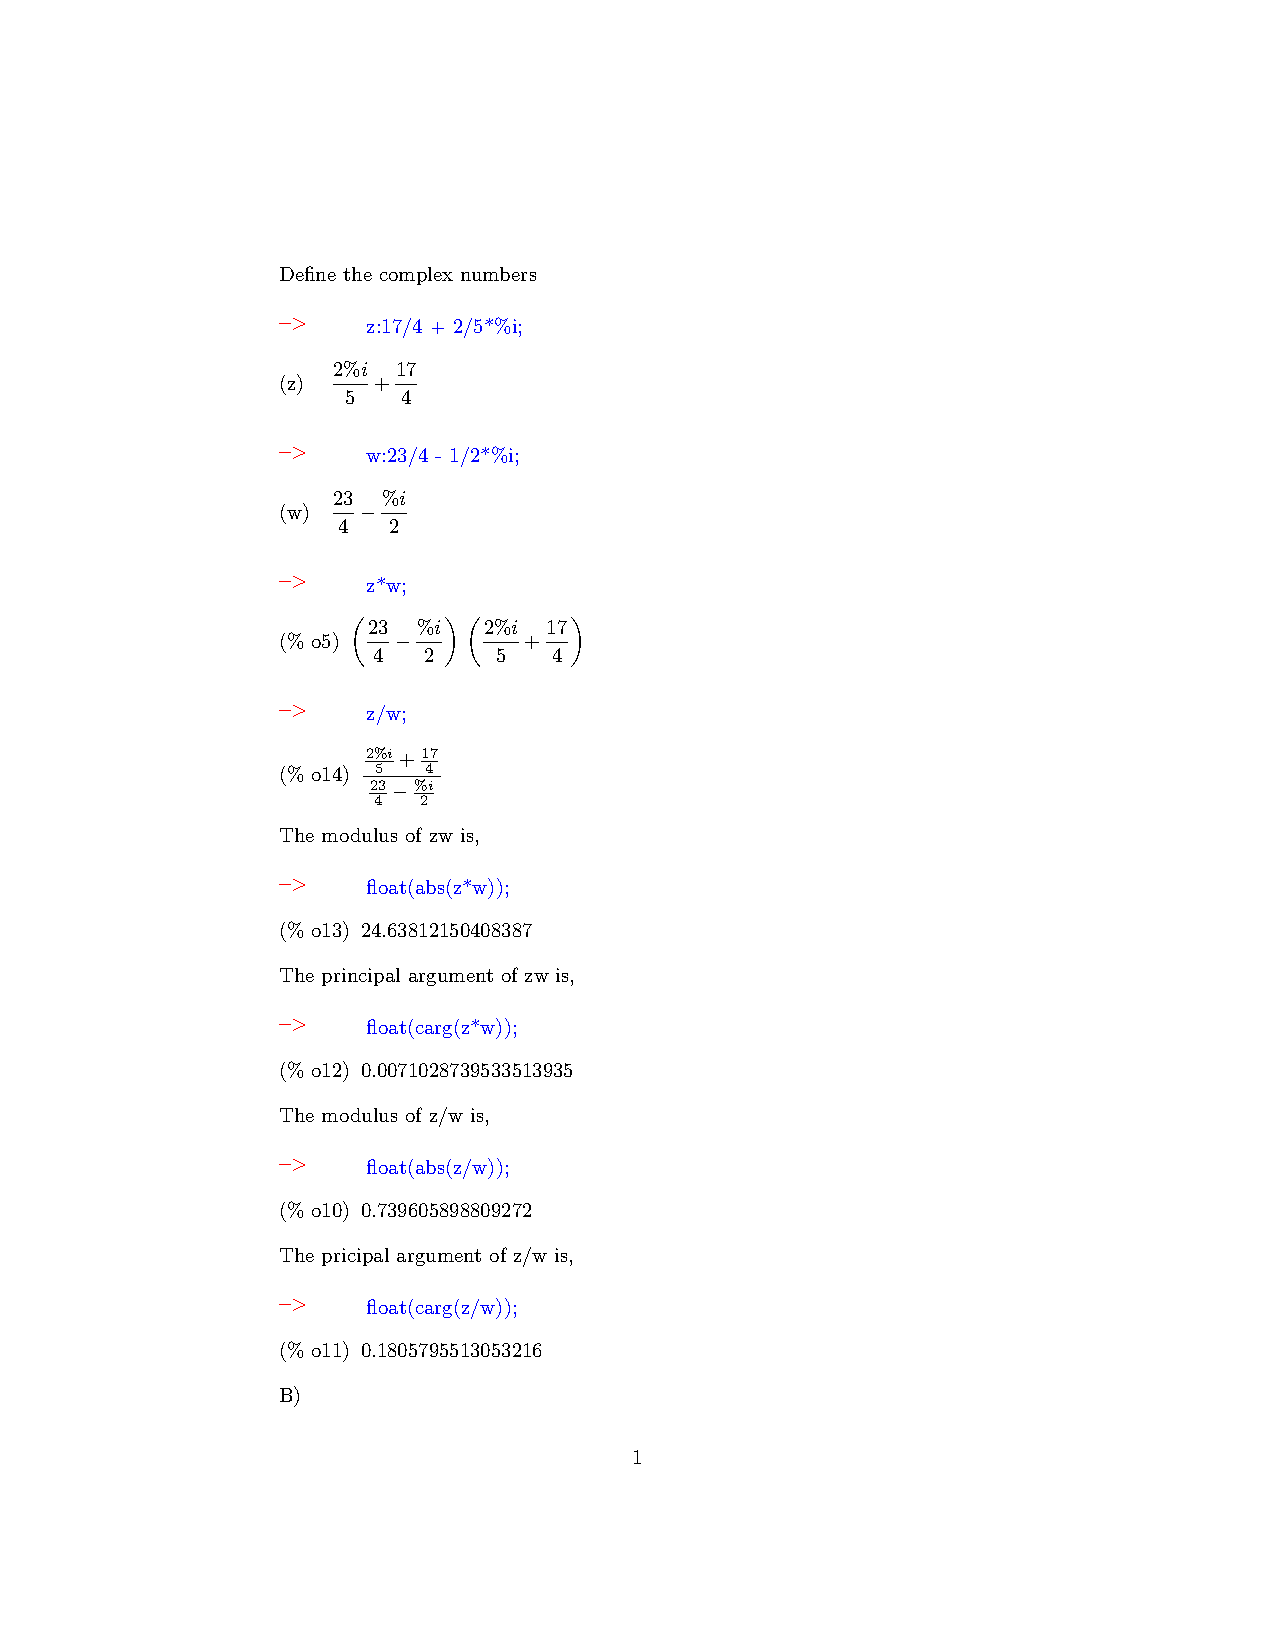
\includepdf[pages=-]{question_10_b.pdf}

\end{question}

\clearpage

%Question eleven

\begin{question}

\qpart

\[ \rb{\frac{2\textit{i}}{3 + 3\sqrt{3}\textit{i}}}^{5} \]

\begin{align*}
\stext{The modulus of the demominator is}\\[8pt]
    \sqrt{3^{2} + 3\sqrt{3}^{2}} &=\\[8pt]
    &= \sqrt{36}\\[8pt]
    &= 6\\[8pt]
\stext{The argument of the denominator is}\\[8pt]
    \taninv\rb{\frac{3\sqrt{3}}{3}} &=\\[8pt]
    &= \taninv{\rb{\sqrt{3}}}\\[8pt]
    &= \frac{\pi}{3}\\[8pt]
\stext{Therefore, in exponetial form}\\[8pt]
    &= 6e^{\textit{i}\frac{\pi}{3}}\\[8pt]
\stext{Express the numerator in exponetial form}\\[8pt]
2\textit{i} &= 2e^{\textit{i}\frac{\pi}{2}}\\[8pt]
\end{align*}

Writing both the numerator and denominator in exponential form

\begin{align*}
    \rb{\frac{2e^{\textit{i}\frac{\pi}{2}}}{6e^{\textit{i}\frac{\pi}{3}}}}^{5} &=\\[8pt]
\stext{Using Index laws}\\[8pt]
    &= \rb{\frac{2}{6}e^{\textit{i}\frac{\pi}{2}-\textit{i}\frac{\pi}{3}}}^5\\[8pt]
    &= \rb{\frac{1}{3}e^{\textit{i}\frac{\pi}{6}}}^5\\[8pt]
\stext{Using De Moivre's formula}\\[8pt]
    &= \rb{\frac{1}{3}}^5e^{\textit{i}\frac{5\pi}{6}}\\[8pt]
    &= \frac{1}{243}e^{\textit{i}\frac{5\pi}{6}}\\[8pt]
\end{align*}

\vspace{5cm}

\qpart

Given
\[\sum_{k=0}^{n=1} \rb{ e^{\frac{2\pi\textit{i}}{n}} }^{k-1} \]

\marginnote{formula for the sum of a geometric series \[ S_{n} = \frac{1-r^{n}}{1-r} \]}

\begin{align*}
\stext{Using the sum of a geometric series}\\[8pt]
    \sum_{k=0}^{n=1}e^{\frac{2\pi\textit{i}}{n}} &= \frac{1-\rb{e^{\frac{2\pi\textit{i}}{n}}}^{n}}{1-e^{\frac{2\pi\textit{i}}{n}}}\\[8pt]
\stext{Using Euler's formula}\\[8pt]
    &= \frac{1-e^{\textit{i}2\pi}}{1-e^{\frac{\textit{i}2\pi}{n}}}\\[8pt]
\stext{From Eulers identity \( e^{2\pi\textit{i}} = 1 \)}\\[8pt]
    &= \frac{1-1}{1-e^{\frac{\textit{i}2\pi}{n}}}\\[8pt]
    &= \frac{0}{1-e^{\frac{\textit{i}2\pi}{n}}}\\[8pt]
    &= 0
\end{align*}

\end{question}

%Question twelve

\begin{question}

    I think my time managment for this module was OK, as I have to get through all the material
    quickly in orer to move on to the next maths module, MST125. And still have enough time to 
    complete the other module in astronomy and prepare for the begining of the IT course that has just started.
    
    I struggled to get to all the tutorials live due to work commitments but always made sure I watched
    as many of the recording as I could.

    I didn't find the forums as useful as I could have because I found I quickly became lost in all the threads because I 
    didn't follow them from the start.

    MAXIMA is a very powerful tool and I found it very useful for checking my answers.
    I still need to put more time into learnig how to use it efficiently, for my upcoming modules.

    My further reading around maths has taken a bit of a back seat whilst I have been trying
    to study basically full time whist also working full time. I hope that next year when my study
    commitments are lestened I will be able to spend more time on this.


\end{question}

%Question thirteen

\begin{question}
    
\end{question}


\end{document}